\section{Related Work (Cont.)}

\paragraph{Autoformalization.} Complementing this line of work, \citet{wang2024theoremLlama} present \textsc{TheoremLlama}, a framework aimed at enhancing LLM translation into Lean 4. Drawing on over 100K proof examples from the Mathlib4 library, TheoremLlama employs a novel natural-language-to-formal-language (NL-FL) bootstrapping strategy and iterative proof synthesis. This enables the reuse of verified examples as templates for future translations. The framework achieves 36.48\% and 33.61\% accuracy on the MiniF2F-Valid and MiniF2F-Test benchmarks, respectively—surpassing GPT-4 by more than ten percentage points on both.

\textbf{Techniques for Code Verification.}
\textsc{ImProver}~\citep{ahuja2024improver} introduces a Lean-aware Chain-of-States prompting loop that integrates retrieval, best-of-$n$ sampling, and iterative correction to rewrite formal proofs with improved properties. By optimizing for metrics such as brevity and readability, ImProver reduces the number of tactics by half, doubles proof readability, and boosts theorem prover acceptance rates by over 80\%.
In addition, \textsc{Clover}~\citep{sun2024clover} implements a closed-loop pipeline in which an LLM first generates code, docstrings, and formal annotations, then uses reconstruction-based prompting to enforce consistency across these outputs, and finally applies SMT-based verification to validate correctness. Evaluated on the CloverBench suite of Dafny programs, Clover accepts 87\% of correct solutions, rejects 100\% of flawed ones, and even uncovers bugs in human-written code—demonstrating the power of hybrid generation-verification pipelines.
In a complementary direction, \citet{zhou2025graders} improve general-purpose LLM-based graders by augmenting them with “privileged” information such as gold-standard solutions, grading rubrics, and detailed annotations. When necessary, the system provides targeted hints back to candidate models. This approach achieves grading performance on par with or exceeding that of specialized systems—and even expert humans—on difficult programming benchmarks.

\textbf{Agentic Frameworks and Tools for Code Verification.}
\textsc{Trace}~\citep{cheng2024trace} proposes \emph{generative optimization}, tuning entire computational workflows—including code, prompts, tool calls, and error signals—by treating execution traces as gradients in the OPTO framework. With a PyTorch-like API and the LLM-based optimizer OptoPrime, it supports diverse tasks such as prompt tuning, debugging, and robot control, rivaling specialized optimizers.
Building on modular composition, \textsc{DSPy}~\citep{khattab2024dspy} treats LLM calls as declarative modules in a computational graph. Users define concise input–output signatures, and DSPy’s compiler automatically bootstraps or fine-tunes pipelines using built-in “teleprompters.” This enables a few-line programs to outperform expert-crafted prompts in math, QA, and agent workflows.
Extending agentic capabilities to formal reasoning, \textsc{Pantograph}~\citep{aniva2025pantograph} offers a programmatic interface to Lean 4 with support for advanced proof search. It exposes internal proof states and tactics for integration with learning agents, replacing human-facing interfaces with API-level control.

% https://gemini.google.com/app/d39eba54ee6763e1
\paragraph{Evaluating Autoformalization with Reference-Free Judges.}
In a complementary line of work, \citet{zhang2025goldstandardsepistemicensemble} propose an ensemble of LLM judges for the autoformalization task, using a fine-grained taxonomy to score formalizations without a gold-standard reference. 
The primary strength of this approach is its reference-free nature, offering a scalable evaluation pathway when gold standards are unavailable or prohibitively expensive to create. 
However, the work's motivation for abandoning gold-standard comparison is based on limited evidence: a small, non-random sample of "potentially incorrect" formalizations pre-selected by an LLM, whose own reliability is uncertified. 
Furthermore, the framework validates its judge by correlating with human preference scores—a subjective proxy—rather than the more objective, machine-checkable goal of logical equivalence to a known-correct specification. 
Critically, even if minor errors exist in gold-standard datasets, recent work has shown that such noise rarely alters the relative ranking of models, as errors are typically correlated across systems \citep{salaudeen2024imagenotcontrastimagenetpreserves}. 
This suggests that a small number of flawed examples does not invalidate the utility of an entire benchmark for comparative evaluation. 
Our work, in contrast, proceeds from the basis that gold standards are sufficiently reliable for ranking and focuses on certifying a judge's logical consistency against them -- which is the desirable gold metric to be using.

\subsection{Related Work: Scalable Oversight}

\paragraph{Scalable Oversight with LLM Judges}
Researchers have proposed multi-agent oversight frameworks such as debate and consultancy, where weaker LLMs act as judges supervising stronger agents \citep{kenton2024oversight,Chan2024ChatEval}. 
Debate, in which two models argue opposing sides before a judge, consistently improves truth-tracking compared to single-pass QA. \citet{kenton2024oversight} demonstrate that debate reduces the likelihood of judges being misled in math and code tasks, highlighting it as a scalable oversight mechanism. 

\paragraph{Self-Improving Critics.}
In the absence of stronger supervisors, models can bootstrap judgment skill through self-critique. 
The Self-Evolving Critic (SCRIT) framework trains LLMs to generate critiques of flawed outputs, validate corrections, and iteratively refine their ability to spot errors. \citet{zheng2024scrit} report improvements of over 10\% on critique benchmarks, showing that self-critique fosters scalable, autonomous oversight.

\paragraph{Certifying Judges.}
Naïve LLM judges are often inconsistent, rewarding stylistic cues over correctness \citep{Kocmi2024HumanVsLLM,Li2024TrustLLMJudgments}. 
% To mitigate this, \citet{anonymous2025formaljudge} propose certifying judges with falsifiable properties. Their Lean-aware theorem judge satisfies both \emph{Identity} (identical inputs yield maximal scores) and \emph{Monotonicity} (scores decrease as bugs or omissions are introduced), with Pearson correlations up to 0.973. This validation enables the judge to serve as a reliable proxy for human evaluation of Lean theorems and specifications.

\paragraph{Validity-Centered Evaluation.}
Certifying judges requires not only behavioral properties but also principled validity evidence. \citet{salaudeen2025measurement} introduce a framework that distinguishes between measurement, claims, and evidence, grounded in psychometrics. They emphasize construct, content, and criterion validity, and systematically enumerate threats to validity. This framework provides a blueprint for reporting and interpreting judge certification results, complementing identity/monotonicity checks with broader validity cards.

\paragraph{Robust Evaluation without Ground Truth.}
Standard judge queries can be brittle in the absence of ground truth, particularly under adversarial manipulation \citep{Zhuo2024ICEScore,TongZhang2024CodeJudge}. \citet{robertson2025stepbystep} model the overseer as an agent and propose using information-theoretic, incentive-compatible queries instead of direct ratings. They introduce bounded $f$-divergence measures such as TVD-MI, which exhibit polynomial robustness to adversarial strategies, unlike unbounded KL-based criteria. This work highlights a pathway toward robust, certifiable judges when explicit ground truth is unavailable.

\paragraph{Formal Methods as Oversight.}
Proof assistants provide binary, kernel-level guarantees. \citet{zhou2024donttrustverify} autoformalize math solutions into Isabelle/HOL and show that filtering via proof checking outperforms majority voting by 12\% on GSM8K. \citet{liu2025safe} extend this approach with SAFE, which verifies every intermediate step in Lean 4 and introduces the FormalStep benchmark, reducing hallucinations and enabling fine-grained oversight.

\paragraph{Agentic Iterative Pipelines.}
\citet{ospanov2023apollo} integrate Lean feedback into recursive repair cycles, boosting general-purpose LLM proof success from 3--7\% to over 40\% on miniF2F, and achieving 75\% with fewer than 1000 samples. \citet{miranda2025veribench} extend this paradigm to program verification, showing that self-debugging agents quadruple success compared to one-shot prompting. 
Incorporating an LLM judge improved completeness on security tasks but required calibration to avoid regressions on simpler cases.

\paragraph{Benchmarks for Judge Reliability.}
Benchmarks such as VeriBench and FormalStep quantify judge reliability across compilation, proof success, and specification quality. 
\citet{miranda2025veribench} report normalized specification scores of 0.470 for one-shot prompting versus 0.615 for self-debugging agents. 
Outside formal mathematics, MT-Bench and G-Eval provide complementary judge-evaluation settings using pairwise preferences and rubric-guided scoring, underscoring the need for calibration and validity reporting \citep{Zheng2023MTBench,Liu2023GEval}. 
Together with validity frameworks and robust information-theoretic scoring, these benchmarks advance the agenda of certifying LLM judges for formal verification.

% https://chatgpt.com/c/68dc36c7-c4b0-8327-9dcd-694c10fa5d93?model=gpt-5-pro
\subsection{HCI for Solving Scalable Oversight}

\paragraph{From more evaluation to \emph{human-centered} oversight.}
HCI reframes scalable oversight as a \emph{calibration} problem: design interactions that let people verify, steer, and place \emph{appropriate} trust in LLM outputs rather than maximizing raw trust \citep{bach2022trusthci}. Interface choices (e.g., citations, explanations, confidence cues) can substantially shift user trust---sometimes in misleading ways---so the goal is to expose process and embed lightweight verification instead of presenting one-shot answers \citep{ding2025citations}. User studies in AI pair-programming similarly surface needs to communicate model performance, provide control over output style/constraints, and expose uncertainty to avoid over-reliance \citep{wang2024trustcode}.%
% :contentReference[oaicite:0]{index=0}

\paragraph{Hybrid human$\leftrightarrow$AI evaluation.}
HCI work operationalizes scalable evaluation by combining expert/lay judgments with automated judges. Humans annotate failures or verify slices of output; systems then train or condition LLM-based ``reference evaluators'' on those signals to scale up assessment while staying anchored to what users value (accuracy, safety, usefulness). This human-in-the-loop pattern complements LLM-as-judge approaches---whose reliability varies by task and setup \citep{Kocmi2024HumanVsLLM,Li2024TrustLLMJudgments}---and is especially relevant when pass@k or single-shot metrics are brittle.%
% :contentReference[oaicite:1]{index=1}

\paragraph{Interfaces that \emph{operationalize} oversight.}
HCI systems instantiate oversight as interaction loops that make correctness checkable \emph{during} generation: (i) \emph{test-driven code generation} (TiCoder) elicits yes/no judgments about candidate unit tests before showing code; a few interactions reduced cognitive effort and lifted pass@1 by $\sim$45.7\% on coding benchmarks \citep{naik2024ticoder}; (ii) \emph{explain$\rightarrow$correct loops} (IntelliExplain) pair each snippet with a natural-language rationale that users can critique, improving novice task success by $\sim$11--25\% \citep{yan2024intelliexplain}; (iii) \emph{pair debugging} (HypoCompass) has humans hypothesize faults while the LLM attempts fixes, yielding $\sim$12\% learning gains \citep{ma2024hypocompass}; (iv) \emph{multi-step pipelines} (PromptChainer) expose intermediate steps (e.g., tests $\rightarrow$ verification $\rightarrow$ proof attempt), enabling user intervention where failures arise \citep{wu2022promptchainer}; and (v) \emph{source-grounded verification} (SymGen) highlights claim-level spans backed by exact sources and leaves unsupported text unhighlighted, speeding verification by $\sim$20\% and raising user confidence \citep{shen2024symgen}. Collectively, these patterns shift trust from fluency to \emph{verifiable progress}.%
% :contentReference[oaicite:2]{index=2}

\paragraph{Applying HCI patterns to formal specs/theorems.}
Formal kernels (Lean/Isabelle) already deliver binary checks; HCI contributes the \emph{workflow glue} that helps users evaluate \emph{which} theorem/spec to prove and whether it is complete. Two actionable patterns: (1) \emph{counterfactual spec probes}---UI toggles that remove a postcondition or inject a known bug and display the impact on tests/judge score---help detect missing clauses or overfitting; and (2) \emph{stepwise proof oversight}---surfacing intermediate goals and marking unverified suggestions---keeps the human in control of proof search. In our setting, these patterns interface naturally with a graded, semantics-sensitive evaluator.%
% :contentReference[oaicite:3]{index=3}

% \paragraph{Complementarity with a \emph{certified} formal judge.}
% \citet{anonymous2025formaljudge} propose certifying an LLM theorem/spec judge via falsifiable properties---\emph{identity} and \emph{monotonicity}---and report strong negative correlations between injected error and score (e.g., $|r|\approx 0.973$) on \textsc{VeriBench} \citep{veribench_icml25}. HCI turns this certified signal into usable oversight by: (a) rendering per-clause rubrics and local confidence hints, (b) exposing the judge’s own sanity checks (identity pairs and monotone ladders) so users see \emph{why} scores move, and (c) attaching a concise \emph{judge card} (intended claim, evidence, threats) in the validity-centered sense of \citet{salaudeen2025measurement}. For settings with weak ground truth or adversaries, information-theoretic overseer queries provide robustness beyond rubric scores \citep{robertson2025stepbystep}.%
% % :contentReference[oaicite:4]{index=4}

% \paragraph{Design takeaways for scalable oversight.}
% \emph{Expose process}, not just outputs (\citealp{wu2022promptchainer}); \emph{facilitate incremental verification} (\citealp{naik2024ticoder,shen2024symgen}); \emph{empower corrective feedback} (\citealp{yan2024intelliexplain}); and \emph{communicate uncertainty honestly} (\citealp{wang2024trustcode,ding2025citations}). These HCI patterns consistently reduce cognitive load, improve objective accuracy, and---critically---align user trust with actual reliability across code/spec/theorem tasks.%
% % :contentReference[oaicite:5]{index=5}

\subsection{Why an LLM judge?}
\citet{bursuc2025benchmarkvericodingformallyverified} presumes well-formed formal specifications and evaluates end-to-end verification under those specs—in Dafny, Verus/Rust, or Lean—reporting verified pass rates. 
In practice, impactful problems often lack both complete specifications and ground-truth answers. 
Our \textsc{VeriBench} program targets this gap by challenging the \emph{generation} of specifications (from code, tests and documentation) and then \emph{certifying} their quality prior to proof search using a Lean-aware LLM judge that we validate via falsifiable principles/properties (Identity and Monotonicity), addressing known pitfalls of LLM-as-a-judge such as bias and prompt sensitivity \citep{Zheng2023MTBench,Kocmi2024HumanVsLLM,Li2024TrustLLMJudgments}. 
However, our framework has only been tested with a judge with gold references files with specifications but we will explore metrics/methods that don't require this like TVD-MI in \citep{robertson2025stepbystep}. 

Beyond spec-first settings, the Unsolved Questions (UQ) paradigm evaluates models on difficult, real-world problems that have neither ground-truth answers nor formal specifications; instead, it relies on validator pipelines and community verification to track progress without oracles \cite{nie2025uqassessinglanguagemodels,uq2025}. 
Taken together, these lines of work shift evaluation from “solve what is already specified” to “specify, certify, then solve”: 
vericoding provides end-to-end rigor under given specs, \textsc{VeriBench} adds specification synthesis with a certified semantic judge, and UQ extends evaluation to specless, answerless settings that require validator-assisted screening. 
Our contribution is a certified, semantics-sensitive judge that enables scalable oversight when the specification must be proposed rather than merely proved. 
Because specification generation often lacks a unique ground truth, we will extend our oracle-free certification protocol with UQ-style validators, adding cycle-consistency tests (spec to code/docs) alongside our bug and ablation ladders, and enabling abstention when validators disagree to prioritize precision over coverage.

\section{Discussion (Cont.)}
\textbf{Why Lean 4?} 
Lean 4 is a full fledge programming language and lets VeriBench contain full runnable code and machine-checked proofs in the same dependently-typed language. 
% \leni{The following sentence should be eliminated. Coq and Isabelle are not inherently less trustworthy}
% This eliminates the extraction gap that separates proof from execution in systems like Coq to OCaml or Isabelle to SML/Scala -- making Lean 4 more trustworthy. 
Ahead-of-time compilation with the Lake toolchain produces fast native binaries, while first-class \texttt{Task} primitives, async I/O, and a thread-pool scheduler enable genuine concurrent programs inside the prover. 
% TODO ([lean-lang.org][1], [lean-lang.org][2])  
Lean’s C-level foreign-function interface (FFI) lets those binaries call out to high-performance libraries when needed. 
% TODO ([docs.lean-lang.org][3], [proofassistants.stackexchange.com][4])  
On the proof side, Lean ships a powerful metaprogramming system written in Lean itself, giving researchers a programming interface to access its internals. This led to the creation of tools such as Pantograph and Aesop.
% ([lean-lang.org][5], [leanprover-community.github.io][6])  
Finally, the community-maintained \texttt{mathlib4} and \texttt{std4} libraries supply thousands of reusable theorems and data structures, and they are expanding quickly thanks to an active Zulip and GitHub ecosystem. Lean also has a work-in-progress program verification library, CSLib, which has recently seen rapid growth.
Lean 4 is backed by an unusually vibrant open-source community: hundreds of contributors refine \texttt{mathlib4} on GitHub each week, the public Zulip sees expert discussion around the clock, and even Fields-Medalist Terence Tao has chosen Lean to formalize portions of his current research—clear testimony to the ecosystem’s accessibility and intellectual depth.
% ([github.com][7], [leanprover-community.github.io][8])
Unlike the unit tests, fuzzers, and code sanitation pipelines common in industry—tools that sample inputs or rely on heuristics—Lean 4 supplies machine-checked proofs that a property holds for \emph{all} executions.  
Its dependent type system can encode deep invariants (e.g., length-indexed arrays, bounded integers), so programs that violate them fail to compile, eliminating whole classes of bugs such as buffer overflows or integer wrap-around. 
Code, specification, and proof reside in the same file and are compiled by Lake into the shipped native binary, preventing the drift that arises when verification artifacts live outside the build. 
% Tactic automation accelerates proof construction while keeping each step inspectable, and Lean’s FFI plus ahead-of-time compilation allow verified components to link with existing C/C++ libraries and run at production speed—even for concurrent tasks handled through built-in async primitives. 
In short, Lean turns informal “best-effort” checks into formal, end-to-end guarantees without sacrificing performance or interoperability.

\textbf{Lean 4’s limitations.}
Lean’s toolchain is still younger than Coq’s or Isabelle’s, making its standard libraries and automation smaller, and thus some formalizations demand extra groundwork. Lean’s runtime has not been stress-tested at the scale of mainstream systems languages, meaning large-scale or safety-critical deployments may require additional vetting. Lean tactics could contain bugs and fail to typecheck on different environments.
Acknowledging these gaps clarifies that VeriBench chooses Lean 4 for its unique unified programming-plus-proving model and modern automation hooks, not because it already matches the decades-old industrial maturity of older theorem provers. 
\noindent\textit{Static vs.\ runtime caveat:}
Lean’s guarantees are \emph{static} and specification‑relative: they certify the Lean program meets the stated properties, but they do not by themselves detect emergent runtime faults outside the model (e.g., I/O (Input/Output) failures, environment misconfiguration, FFI (Foreign Function Interface) unsoundness, resource exhaustion, or undefined behavior in linked C code). 
Such behaviors must either be modeled and proved, or mitigated with production safeguards (monitoring, sandboxing, input validation).

% [1]: https://lean-lang.org/doc/reference/latest/IO/Tasks-and-Threads/?utm_source=chatgpt.com "15.11. Tasks and Threads - Lean"
% [2]: https://lean-lang.org/doc/reference/4.19.0/Build-Tools-and-Distribution/Lake/?utm_source=chatgpt.com "Lake - Lean"
% [3]: https://docs.lean-lang.org/lean4/doc/dev/ffi.html?utm_source=chatgpt.com "Foreign Function Interface - Lean Documentation Overview"
% [4]: https://proofassistants.stackexchange.com/questions/4445/lean-4-foreign-function-interface-for-matrix-multiplication?utm_source=chatgpt.com "lean 4 foreign function interface for matrix multiplication?"
% [5]: https://lean-lang.org/doc/reference/latest/Notations-and-Macros/Macros/?utm_source=chatgpt.com "19.5. Macros - Lean"
% [6]: https://leanprover-community.github.io/lean4-metaprogramming-book/main/06_macros.html?utm_source=chatgpt.com "Macros - Metaprogramming in Lean 4"
% [7]: https://github.com/leanprover-community/mathlib4?utm_source=chatgpt.com "leanprover-community/mathlib4: The math library of Lean 4 - GitHub"
% [8]: https://leanprover-community.github.io/mathlib4_docs/index.html?utm_source=chatgpt.com "Mathlib Documentation - Lean community"

\textbf{Lean 4 versus Dafny.}  
Unlike Dafny, whose verifier translates each program into the Boogie intermediate language and then discharges first-order verification conditions with an SMT solver such as Z3, Lean 4 reasons natively in a dependently-typed calculus. 
% ([leino.science][1], [dafny.org][2])  
Because Lean 4’s types can mention run-time data and the very same source code is ahead-of-time compiled to a native binary via Lake, we can both state and prove value-indexed, higher-order properties (e.g., length-indexed vectorsand run the verified program itself—an end-to-end, fidelity that Dafny’s SMT-centred, Boogie-to-Z3 workflow cannot natively match.  
This gives Lean the expressive power to specify and prove higher-order, data-dependent properties—precisely the kind of semantic guarantees VeriBench seeks to test—while still yielding runnable binaries compiled by the same toolchain. 
Dafny’s SMT-centric workflow offers impressive push-button automation for imperative code but cannot natively encode the richer specifications (e.g., length-indexed vectors, algebraic invariants) that Lean handles directly. 
% ([lean-lang.org][3])

% [1]: https://leino.science/papers/krml221.pdf?utm_source=chatgpt.com "[PDF] Using Dafny, an Automatic Program Verifier - Rustan Leino"
% [2]: https://dafny.org/dafny/DafnyRef/DafnyRef.html?utm_source=chatgpt.com "Dafny Documentation"
% [3]: https://lean-lang.org/theorem_proving_in_lean4/dependent_type_theory.html?utm_source=chatgpt.com "Dependent Type Theory - Theorem Proving in Lean 4"

\textbf{Lean 4 versus TLA+.} 
TLA+ excels at high-level specification of concurrent and distributed protocols, with correctness checked by the TLC model-checker and the TLAPS proof system that dispatches first-order obligations to external provers. % ([lamport.azurewebsites.net][1], [proofs.tlapl.us][2], [lamport.azurewebsites.net][3])  
However, TLA+ specifications are not executable programs; a separate implementation step is required, and state-space explosion can limit model-checking scalability. 
VeriBench instead needs a prover where the specification, proof, and runnable code live in the same language. 
Lean 4’s dependently-typed core lets us capture fine-grained, data-dependent invariants and then compile the very same artifacts to fast native binaries—capabilities outside TLA+’s scope. 

\textbf{Lean 4 verus Verus.}
Verus is a verification framework for Rust programs using SMT solvers. A user state intermediate goals and an SMT backend fills in the intermediate steps. Compared to Verus, users have the option to use or not use SMT Solver-based tactics in Lean. This enables more fine-grained control and steering of the proof process. Verus also has a much larger kernel compared to Lean, and is more susceptible to soundness problem than Lean whose kernel is small.

\section{Future Work (cont.)}

% https://chatgpt.com/c/68dc38a5-93f4-8322-bf91-c2802fe73f6f
While \citep{robertson2025stepbystep} study demonstrates that total-variation-based mutual information (TVD-MI) provides robust, gaming-resistant evaluation without ground truth, many settings —such as VeriBench— do provide gold specifications in Lean 4. 
A promising direction is to develop hybrid protocols that combine TVD-MI’s black-box robustness with supervised ground-truth checks (compile success, unit tests, post-condition proofs, and equivalence theorems). 
By calibrating MI scores against known gold outcomes, we can create composite metrics that preserve gaming-resistance while offering calibrated probabilities of correctness where supervision exists. 
This opens the door to semi-supervised label propagation, active selection of items to prove, and cross-system experiments in domains with heterogeneous supervision.
Such an integration would extend Robertson’s information-theoretic framework into a practical, specification-aware oversight system that leverages the best of both unsupervised robustness and supervised precision.

\section{Why Judge Scores Are Specification-Relative}

It is tempting to interpret a perfect score from our LLM judge as a guarantee of absolute program correctness. However, this is fundamentally impossible due to established limits from computability theory. The obstacle is not a lack of ingenuity in our benchmark design or judge prompting, but an established negative result.

\paragraph{Rice’s Theorem.}
The core limitation stems from Rice’s theorem, which states that any non-trivial, semantic property of programs in a Turing-complete language is undecidable.

\begin{quote}
  \textbf{Rice's Theorem (Informal):} Let $\mathcal{S}$ be any property of a program's input-output behavior (e.g., "the program always terminates" or "the output is always sorted"). If $\mathcal{S}$ is non-trivial (meaning some programs have it and some don't), then no algorithm can exist that decides for \emph{every} program whether it satisfies $\mathcal{S}$.
\end{quote}

\paragraph{Impact on the Gold Standard and the Judge.}
Rice's theorem directly implies that the gold reference files used by our judge are necessarily incomplete. If a recursively enumerable gold standard could capture \emph{every} true semantic property of a program, one could use it to build a decision procedure that contradicts the theorem. Therefore, our gold standards, while rigorous, represent a curated but fundamentally finite set of important specifications.

This leads to a critical conclusion for our work: the judge's evaluation is **specification-relative**. A perfect score does not certify universal semantic correctness; rather, it certifies perfect **conformance to our specific gold standard**. Acknowledging this limitation is essential for correctly interpreting the judge's scores and understanding the scope of our evaluation.


\section{Judge Certification: Additional Plots}\label{app:judge-cert}
We report raw scatterplots used during certification of the LLM judge. These plots visualize the judge’s response to controlled perturbations: (P1) identity/reflexivity, (P2) cumulative bug injection, and (P3) removal of specification items (tests/theorems). Figures A.1–A.3 show that scores drop as artifacts worsen; the bug plot is noisier with an early prompt, which motivated the simplified rubric used in the main experiments.

\textit{Protocol variants.} The scatterplots below are “sanity-check” runs with the simplest prompts to stress visible monotonic behavior. In the bug study (Fig.~\ref{fig:app-bugs}) the earlier, theorem-equivalence prompt produced a noisier trend; this prompted a simplified, rubric-first prompt that we use for all reported results in the main paper, yielding the stronger correlations cited in Fig.~\ref{fig:judge_sanity_checks}. For missing-specs (Fig.~\ref{fig:app-missing-specs}), both Claude 3.5 and 3.7 show clear negative trends; minor non-monotonicity in 3.7 disappears with the finalized rubric.

We note that, for the experiment shown in Figure \ref{fig:app-missing-specs}, a more complex judge (Claude 3.7) does not satisfy the property that the LLM Judge Score should monotonically increase with the number of missing specs. Indeed, the Judge File Equivalence score was not monotonic, even for Claude 3.5, leading us to simplify the rubric used in our main paper.

\begin{figure*}[t]
  \centering
  \begin{subfigure}[t]{0.48\textwidth}
    \centering
    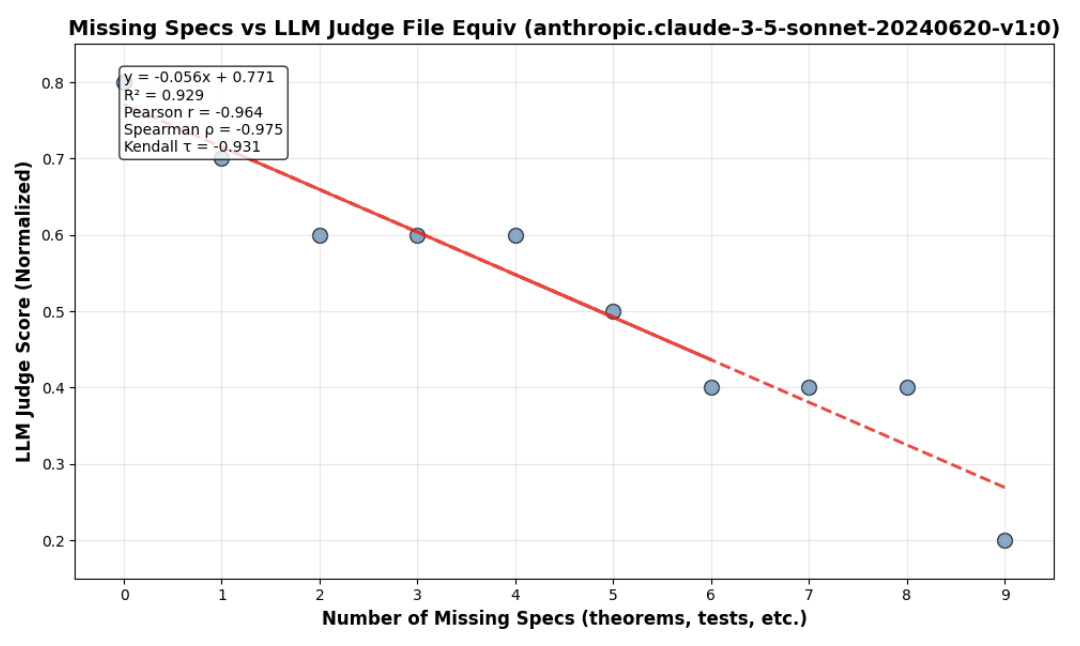
\includegraphics[width=\linewidth]{figures/3.5_specs_missing.png}
    \caption{Claude 3.5 Sonnet v1: strong monotonic decrease (\(y=-0.056x+0.771\), \(R^2=0.929\), Pearson \(r=-0.964\), Spearman \(\rho=-0.975\)).}
  \end{subfigure}\hfill
  \begin{subfigure}[t]{0.48\textwidth}
    \centering
    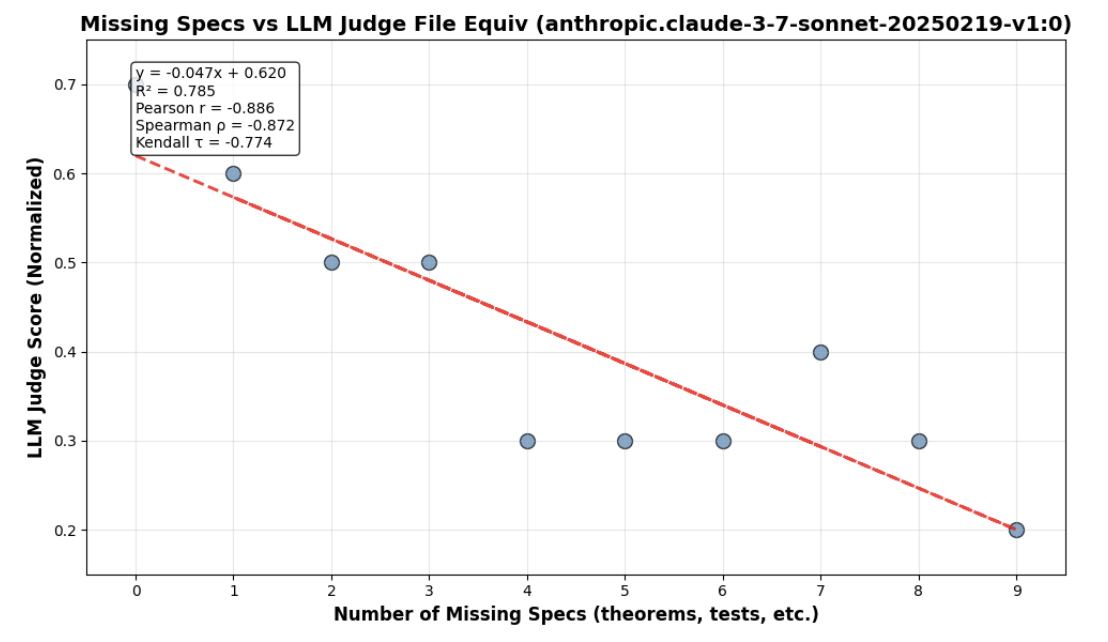
\includegraphics[width=\linewidth]{figures/3.7_specs_missing.png}
    \caption{Claude 3.7 Sonnet v1: clear negative trend with minor non-monotonicity (\(y=-0.047x+0.620\), \(R^2=0.785\), Pearson \(r=-0.886\), Spearman \(\rho=-0.872\)).}
  \end{subfigure}
  \caption{\textbf{(P3) Monotonicity w.r.t.\ missing specifications.}
  Candidate scores decrease as more theorems/tests are withheld. We retain both model variants to show robustness of the trend; 3.7’s small non-monotonicity motivated the simplified rubric used in the main results.}
  \label{fig:app-missing-specs}
\end{figure*}

\begin{figure}[t]
  \centering
  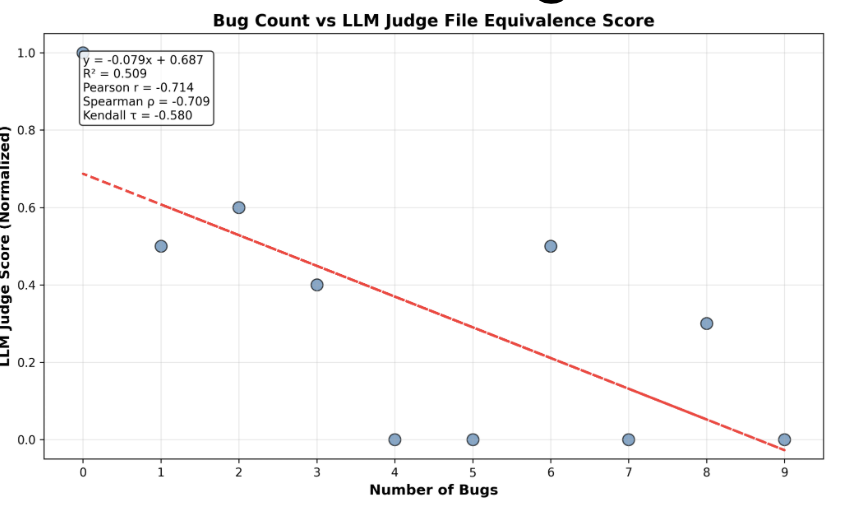
\includegraphics[width=0.85\linewidth]{figures/3.5_bugs.png}
  \caption{\textbf{(P2) Non-Monotonicity w.r.t.\ cumulative bugs (Claude 3.5 Sonnet).}
  Scores drop as more semantic bugs are injected (Pearson \(r=-0.714\), Spearman \(\rho=-0.709\), \(R^2=0.509\)); the higher noise with the initial “theorem-equivalence” prompt led us to simplify the rubric used for the final judge in the main paper.}
  \label{fig:app-bugs}
\end{figure}